% ----------------------------------------------------------
\chapter{Introdução}\label{cap:intro}
% ----------------------------------------------------------

% A contagem de polígonos em artefatos gráficos em filmes, jogos, pesquisas medicas e cientificas seguem em crescimento
% vertiginosa e apesar do Hardware acompanhar este crescimento, existem claras restrições com relação a V-RAM e a
% RAM. Com essas restrições em mente, são necessárias estruturas de dados que permitam o acesso rápido dessas
% figuras, consultas e armazenamento.
% A seleção e determinação de faces visíveis VSD.
A cada nova geração de consoles, desenvolvedores e artistas gráficos aumentam a  qualidade gráfica incrementando a contagem de polígonos em cada objeto 3D\footnote{A cada geração a contagem de polígonos chega a quintuplicar \url{https://blog.playstation.com/2019/12/16/the-polygonal-evolution-of-5-iconic-playstation-characters/}}. Com objetos tridimensionais e cenas cada vez mais complexas, sendo jogos aplicações de tempo real, se faz necessário que os algoritmos realizem consultas a esses objetos rapidamente pois o tempo da consulta não pode extrapolar o tempo limite esperado para desenhar cada quadro da aplicação.
Este trabalho visa apresentar estruturas de dados conhecidas que auxiliem a evolução do hardware a fim de produzir consultas aos objetos e figuras geométricas de forma eficiente. Sabemos que cada objeto tridimensional é composto de figuras simples como triângulos, vértices e arestas \cite{opengl}. Portanto, se pudermos consultar tais figuras de forma eficiente, poderemos estender para uma aplicação tridimensional pois podemos decompor em segmentos de reta, ou ainda em pontos. O nosso trabalho considera a decomposição de polígonos sobre estes dois objetos geométricos mais simples: pontos e segmentos de reta.

Ao longo deste trabalho iremos ver estruturas de dados para consultar pontos bidimensionais que podem ser facilmente estendidas para três dimensões e utilizadas assim para jogos tridimensionais. O objetivo de consultas rápidas pode ser variado: consultar quais objetos devem ser desenhados sem o custo de consultar linearmente quais objetos estão presentes dentro do raio da câmera. Permitindo construção de grandes cenas sem um grande custo de consulta. Podemos utilizar também para otimizar algoritmos que preenchem triângulos \footnote{Podemos enviar para a V-RAM apenas o que a nossa consulta retornar \url{https://www.khronos.org/opengl/wiki/Rendering_Pipeline_Overview}} informando para o pipeline gráfico apenas os vértices dentro da consulta \cite{opengl}. Estudamos árvore $KD$ que subdivide o espaço em cada $K$ dimensões permitindo consultas espaciais.% e, para este trabalho focamos em consultas em janela nesta árvore, onde mostramos que no pior caso, é uma consulta linear. 
Em seguida, estudamos árvores de alcance, sendo esta uma árvore binária balanceada multinível. Isto é, cada nó da árvore tem uma outra árvore anexa representando outra dimensão. Sua construção é pensada em fazer consultas em intervalos, sendo uma estrutura eficiente para consultas em janela. Em seguida vemos árvores de intervalo que permite consultas de segmentos paralelos aos eixos de uma janela. Podendo esta ser utilizada para consulta de objetos considerando apenas suas grandezas espaciais. E por fim, estudaremos árvores de segmentos, que permite a consulta de segmentos com quaisquer inclinação. %Podemos então consultar se qualquer segmento está em uma janela.

As nossas implementações foram aplicadas em dois cenários. No primeiro, temos um conjunto de pontos no plano que representam objetos em um mapa e um outro ponto que percorre esse mapa e assim, deslocando a janela pelo mapa. No segundo, temos um conjunto de segmentos no plano que descrevem o mapa do Brasil, fixamos um ponto no mapa, definimos uma janela a partir deste ponto e desenhamos somente aqueles segmentos do mapa que estão na janela.

% ----------------------------------------------------------
%\section{Objetivos}
% ----------------------------------------------------------




% % ----------------------------------------------------------
% % Introdução (exemplo de capítulo sem numeração, mas presente no Sumário)
% % ----------------------------------------------------------
%\chapter*[Introdução]{Introdução}
%\addcontentsline{toc}{chapter}{Introdução}
% % ----------------------------------------------------------

Para introduzirmos o assunto de consulta por figuras geométricas iremos passar uma visão geral das estruturas estudadas e sobre computação gráfica, pois este é o nosso objetivo fim.

\section{Árvores binária de busca balanceada}
Neste trabalho estudamos árvores binária de busca especiais para objetos geométricos. Uma árvore binária é uma estrutura de dados que possui nós e arestas. Alguns nós são internos, enquanto que outros são folhas. Os nós internos possuem no máximo dois filhos e os nós folhas não possuem filhos. Supondo chaves armazenadas em cada nó e em árvores de busca, os nós das subárvores à esquerda tem valores menores ou iguais à chave do nó pai. E, respectivamente, as subárvores à direita tem chaves maiores que a do nó pai. O ideal em uma árvore binária de busca é estruturar dados de forma que seja eficiente uma consulta por uma chave. A construção dá-se dado um conjunto de valores $S = {x_1, x_2, ... x_n}$, constrói-se um nó e chama-se raiz $v$. Guardamos o primeiro valor $x_1$ neste nó. Obtemos o próximo valor $x_2$ comparamos com o valor da raiz $v$, caso seja $x_2 < v = x_1$, criamos um novo nó guardamos o valor de $x_2$ neste nó e inserimos na subárvore à esquerda de $v$. Reciprocamente caso operamos com $x_2 > v = x_1$, inserimos o novo nó em uma subárvore à direita de $v$. Obtemos o próximo valor $x_3$ e este é $x_3 > v = x_1$. Portanto inserimos à direita de $v$. Seguimos assim até $x_n$. 

\begin{figure}[h]
\centering
\resizebox{.2\textwidth}{!}{
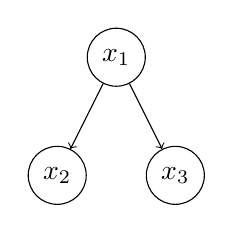
\begin{tikzpicture}[nodes={draw, circle}, ->]
 \node{$x_1$}
    child { 
    node{$x_2$}
    }
    child {
    node {$x_3$}
    };

\end{tikzpicture}
}
\caption{Árvore binária exemplo}
\label{fig:14}
\end{figure}

É importante dizer que a construção de uma árvore binária de busca desta forma não garante que uma consulta na árvore será feita de forma eficiente. Para isso, existem outros algoritmos que podem rotacionar subárvores de tal forma que garanta sempre uma altura "ótima" para a árvore.  Logo descreveremos sobre árvores binária de busca balanceadas.

A consulta em uma árvore pode ser feita de através de chamadas recursivas, onde dado um valor de consulta $s$, compara o valor do nó $v$ com o valor $s$. Caso $s > v$, isto implica que a consulta deve seguir pela subárvore à direita de $v$. Simetricamente, caso $s < v$ implica que a consulta deve seguir pela subárvore esquerda, fazendo uma chamada recursiva com os respectivos nós das subárvores determinadas pela comparação. A condição de parada da consulta é se $s = v$, ou se a árvore é vazia.

Uma árvore binária de busca é dita balanceada quando a altura da árvore é da ordem $\log_{2}{n}$ para uma árvore com $n$ elementos. Uma árvore binária de busca não necessariamente está balanceada. Uma árvore que não esteja balanceada pode ter, nos piores casos de uma consulta, tempo de consulta igual o de uma lista. Ou seja, uma consulta linear e portanto perdendo as qualidades de uma árvore de busca. Existem técnicas para evitar que isso aconteça. A que usamos para atingir este fim neste estudo é pre-ordenar o conjunto de valores (chaves) a serem inseridos na árvore. Isto garante que a árvore que será construída será balanceada \cite{cormen1}.

\section{Computação Gráfica}\label{cap:cg}
Afim de compreendermos as implicações e como podemos utilizar as estruturas usadas em jogos e em aplicações gráficas de tempo real queremos ter uma ideia básica de onde podemos utilizar as estruturas de dados. O componente central de um sistema de gráficos em tempo real é o que se chama de pipeline gráfico representado na Figura \ref{fig:graphical_pipeline}. 

\begin{figure}[h!]
    \centering
    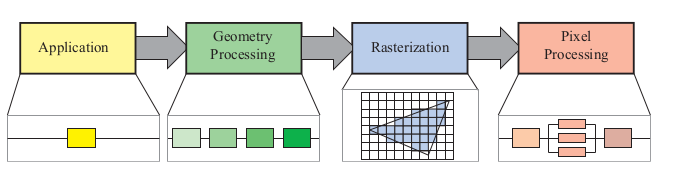
\includegraphics[scale=0.5]{images/Captura de tela de 2021-04-16 19-23-57.png}
    \caption{\cite{rtr1} Pipeline gráfico para renderização de imagens em tempo real}
    \label{fig:graphical_pipeline}
\end{figure}

Sua principal função é desenhar uma imagem bidimensional na tela, dado objetos tridimensionais, uma câmera, fontes de iluminação, etc. O tempo de desenho de cada quadro é expresso por \emph{Quadros Por Segundo} (QPS), isto é, a quantidade de quadros produzidos a cada segundo. No primeiro estágio, \emph{aplicação} é onde o programa lógico da aplicação está sendo executado, por exemplo, checagem de colisão, simulação de física, animação e outros. O estágio seguinte é o \emph{processamento de geometria} que lida com as transformações geométricas, projeções, como um objeto (\emph{vertex shader}) vai ser desenhado e onde vai ser desenhado. O estágio de \emph{rasterização} toma como entrada três vértices de um triângulo, encontra todos os pixel que definem este triângulo e executa um programa (\emph{fragment shader}) para cada pixel determinando sua cor. Finalmente, o \emph{processamento por pixel} executa um programa por pixel para determinar se é visível ou não, além de outros artifícios para coloração. O desenvolvedor tem total domínio dos triângulos que serão desenhados já no estágio de aplicação. Podendo realizar consultas em nível de aplicação e entregar os pontos para o estágio de \emph{processamento de geometria} somente os pontos que consultamos.

\begin{figure}[h!]
    \centering
    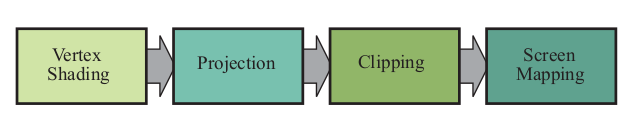
\includegraphics[scale=0.5]{images/Captura de tela de 2021-04-16 19-49-28.png}
    \caption{Estágio de geometria subdividido}
    \label{fig:geometry_pipeline}
\end{figure}

Sabemos que o estágio de geometria executa um algoritmo chamado \emph{recorte (clipping)}, que recorta os segmentos que estão fora da janela visível, desenhando somente o que está dentro da janela. Porém, o algoritmo será aplicado a todos os vértices que foram enviados para o pipeline. Além disso, o maior gargalo em uma das partes do pipeline atrasa todo o resto do processamento gráfico. Portanto, com nossas estruturas de dados conseguiremos deixar eficiente não só o processamento de geometria por ter os pontos dentro da janela a ser trabalhada como por consequência otimizaremos o resto de todo o pipeline. Em seguida, iniciamos nossa apresentação dos algoritmos e estruturas de dados estudados. 